% Options for packages loaded elsewhere
% Options for packages loaded elsewhere
\PassOptionsToPackage{unicode}{hyperref}
\PassOptionsToPackage{hyphens}{url}
\PassOptionsToPackage{dvipsnames,svgnames,x11names}{xcolor}
%
\documentclass[
  letterpaper,
  DIV=11,
  numbers=noendperiod]{scrartcl}
\usepackage{xcolor}
\usepackage{amsmath,amssymb}
\setcounter{secnumdepth}{-\maxdimen} % remove section numbering
\usepackage{iftex}
\ifPDFTeX
  \usepackage[T1]{fontenc}
  \usepackage[utf8]{inputenc}
  \usepackage{textcomp} % provide euro and other symbols
\else % if luatex or xetex
  \usepackage{unicode-math} % this also loads fontspec
  \defaultfontfeatures{Scale=MatchLowercase}
  \defaultfontfeatures[\rmfamily]{Ligatures=TeX,Scale=1}
\fi
\usepackage{lmodern}
\ifPDFTeX\else
  % xetex/luatex font selection
\fi
% Use upquote if available, for straight quotes in verbatim environments
\IfFileExists{upquote.sty}{\usepackage{upquote}}{}
\IfFileExists{microtype.sty}{% use microtype if available
  \usepackage[]{microtype}
  \UseMicrotypeSet[protrusion]{basicmath} % disable protrusion for tt fonts
}{}
\makeatletter
\@ifundefined{KOMAClassName}{% if non-KOMA class
  \IfFileExists{parskip.sty}{%
    \usepackage{parskip}
  }{% else
    \setlength{\parindent}{0pt}
    \setlength{\parskip}{6pt plus 2pt minus 1pt}}
}{% if KOMA class
  \KOMAoptions{parskip=half}}
\makeatother
% Make \paragraph and \subparagraph free-standing
\makeatletter
\ifx\paragraph\undefined\else
  \let\oldparagraph\paragraph
  \renewcommand{\paragraph}{
    \@ifstar
      \xxxParagraphStar
      \xxxParagraphNoStar
  }
  \newcommand{\xxxParagraphStar}[1]{\oldparagraph*{#1}\mbox{}}
  \newcommand{\xxxParagraphNoStar}[1]{\oldparagraph{#1}\mbox{}}
\fi
\ifx\subparagraph\undefined\else
  \let\oldsubparagraph\subparagraph
  \renewcommand{\subparagraph}{
    \@ifstar
      \xxxSubParagraphStar
      \xxxSubParagraphNoStar
  }
  \newcommand{\xxxSubParagraphStar}[1]{\oldsubparagraph*{#1}\mbox{}}
  \newcommand{\xxxSubParagraphNoStar}[1]{\oldsubparagraph{#1}\mbox{}}
\fi
\makeatother

\usepackage{color}
\usepackage{fancyvrb}
\newcommand{\VerbBar}{|}
\newcommand{\VERB}{\Verb[commandchars=\\\{\}]}
\DefineVerbatimEnvironment{Highlighting}{Verbatim}{commandchars=\\\{\}}
% Add ',fontsize=\small' for more characters per line
\usepackage{framed}
\definecolor{shadecolor}{RGB}{241,243,245}
\newenvironment{Shaded}{\begin{snugshade}}{\end{snugshade}}
\newcommand{\AlertTok}[1]{\textcolor[rgb]{0.68,0.00,0.00}{#1}}
\newcommand{\AnnotationTok}[1]{\textcolor[rgb]{0.37,0.37,0.37}{#1}}
\newcommand{\AttributeTok}[1]{\textcolor[rgb]{0.40,0.45,0.13}{#1}}
\newcommand{\BaseNTok}[1]{\textcolor[rgb]{0.68,0.00,0.00}{#1}}
\newcommand{\BuiltInTok}[1]{\textcolor[rgb]{0.00,0.23,0.31}{#1}}
\newcommand{\CharTok}[1]{\textcolor[rgb]{0.13,0.47,0.30}{#1}}
\newcommand{\CommentTok}[1]{\textcolor[rgb]{0.37,0.37,0.37}{#1}}
\newcommand{\CommentVarTok}[1]{\textcolor[rgb]{0.37,0.37,0.37}{\textit{#1}}}
\newcommand{\ConstantTok}[1]{\textcolor[rgb]{0.56,0.35,0.01}{#1}}
\newcommand{\ControlFlowTok}[1]{\textcolor[rgb]{0.00,0.23,0.31}{\textbf{#1}}}
\newcommand{\DataTypeTok}[1]{\textcolor[rgb]{0.68,0.00,0.00}{#1}}
\newcommand{\DecValTok}[1]{\textcolor[rgb]{0.68,0.00,0.00}{#1}}
\newcommand{\DocumentationTok}[1]{\textcolor[rgb]{0.37,0.37,0.37}{\textit{#1}}}
\newcommand{\ErrorTok}[1]{\textcolor[rgb]{0.68,0.00,0.00}{#1}}
\newcommand{\ExtensionTok}[1]{\textcolor[rgb]{0.00,0.23,0.31}{#1}}
\newcommand{\FloatTok}[1]{\textcolor[rgb]{0.68,0.00,0.00}{#1}}
\newcommand{\FunctionTok}[1]{\textcolor[rgb]{0.28,0.35,0.67}{#1}}
\newcommand{\ImportTok}[1]{\textcolor[rgb]{0.00,0.46,0.62}{#1}}
\newcommand{\InformationTok}[1]{\textcolor[rgb]{0.37,0.37,0.37}{#1}}
\newcommand{\KeywordTok}[1]{\textcolor[rgb]{0.00,0.23,0.31}{\textbf{#1}}}
\newcommand{\NormalTok}[1]{\textcolor[rgb]{0.00,0.23,0.31}{#1}}
\newcommand{\OperatorTok}[1]{\textcolor[rgb]{0.37,0.37,0.37}{#1}}
\newcommand{\OtherTok}[1]{\textcolor[rgb]{0.00,0.23,0.31}{#1}}
\newcommand{\PreprocessorTok}[1]{\textcolor[rgb]{0.68,0.00,0.00}{#1}}
\newcommand{\RegionMarkerTok}[1]{\textcolor[rgb]{0.00,0.23,0.31}{#1}}
\newcommand{\SpecialCharTok}[1]{\textcolor[rgb]{0.37,0.37,0.37}{#1}}
\newcommand{\SpecialStringTok}[1]{\textcolor[rgb]{0.13,0.47,0.30}{#1}}
\newcommand{\StringTok}[1]{\textcolor[rgb]{0.13,0.47,0.30}{#1}}
\newcommand{\VariableTok}[1]{\textcolor[rgb]{0.07,0.07,0.07}{#1}}
\newcommand{\VerbatimStringTok}[1]{\textcolor[rgb]{0.13,0.47,0.30}{#1}}
\newcommand{\WarningTok}[1]{\textcolor[rgb]{0.37,0.37,0.37}{\textit{#1}}}

\usepackage{longtable,booktabs,array}
\usepackage{calc} % for calculating minipage widths
% Correct order of tables after \paragraph or \subparagraph
\usepackage{etoolbox}
\makeatletter
\patchcmd\longtable{\par}{\if@noskipsec\mbox{}\fi\par}{}{}
\makeatother
% Allow footnotes in longtable head/foot
\IfFileExists{footnotehyper.sty}{\usepackage{footnotehyper}}{\usepackage{footnote}}
\makesavenoteenv{longtable}
\usepackage{graphicx}
\makeatletter
\newsavebox\pandoc@box
\newcommand*\pandocbounded[1]{% scales image to fit in text height/width
  \sbox\pandoc@box{#1}%
  \Gscale@div\@tempa{\textheight}{\dimexpr\ht\pandoc@box+\dp\pandoc@box\relax}%
  \Gscale@div\@tempb{\linewidth}{\wd\pandoc@box}%
  \ifdim\@tempb\p@<\@tempa\p@\let\@tempa\@tempb\fi% select the smaller of both
  \ifdim\@tempa\p@<\p@\scalebox{\@tempa}{\usebox\pandoc@box}%
  \else\usebox{\pandoc@box}%
  \fi%
}
% Set default figure placement to htbp
\def\fps@figure{htbp}
\makeatother





\setlength{\emergencystretch}{3em} % prevent overfull lines

\providecommand{\tightlist}{%
  \setlength{\itemsep}{0pt}\setlength{\parskip}{0pt}}



 


\KOMAoption{captions}{tableheading}
\makeatletter
\@ifpackageloaded{caption}{}{\usepackage{caption}}
\AtBeginDocument{%
\ifdefined\contentsname
  \renewcommand*\contentsname{Table of contents}
\else
  \newcommand\contentsname{Table of contents}
\fi
\ifdefined\listfigurename
  \renewcommand*\listfigurename{List of Figures}
\else
  \newcommand\listfigurename{List of Figures}
\fi
\ifdefined\listtablename
  \renewcommand*\listtablename{List of Tables}
\else
  \newcommand\listtablename{List of Tables}
\fi
\ifdefined\figurename
  \renewcommand*\figurename{Figure}
\else
  \newcommand\figurename{Figure}
\fi
\ifdefined\tablename
  \renewcommand*\tablename{Table}
\else
  \newcommand\tablename{Table}
\fi
}
\@ifpackageloaded{float}{}{\usepackage{float}}
\floatstyle{ruled}
\@ifundefined{c@chapter}{\newfloat{codelisting}{h}{lop}}{\newfloat{codelisting}{h}{lop}[chapter]}
\floatname{codelisting}{Listing}
\newcommand*\listoflistings{\listof{codelisting}{List of Listings}}
\makeatother
\makeatletter
\makeatother
\makeatletter
\@ifpackageloaded{caption}{}{\usepackage{caption}}
\@ifpackageloaded{subcaption}{}{\usepackage{subcaption}}
\makeatother
\usepackage{bookmark}
\IfFileExists{xurl.sty}{\usepackage{xurl}}{} % add URL line breaks if available
\urlstyle{same}
\hypersetup{
  pdftitle={Bilanci imprese - ratios regionali},
  pdfauthor={Paolo Volterra},
  pdfkeywords={bilanci, imprese, Bankit, indici, ratios, leverage, ROE, ROA, PFN, patrimonializzazione, mezzipropri, indebitamento},
  colorlinks=true,
  linkcolor={blue},
  filecolor={Maroon},
  citecolor={Blue},
  urlcolor={Blue},
  pdfcreator={LaTeX via pandoc}}


\title{Bilanci imprese - ratios regionali}
\usepackage{etoolbox}
\makeatletter
\providecommand{\subtitle}[1]{% add subtitle to \maketitle
  \apptocmd{\@title}{\par {\large #1 \par}}{}{}
}
\makeatother
\subtitle{Analisi per area geografica basata su dati 2018-2023 Banca
d'Italia}
\author{Paolo Volterra}
\date{}
\begin{document}
\maketitle

La collana
\href{https://www.bancaditalia.it/pubblicazioni/economie-regionali/index.html}{Economie
regionali} di banca d'Italia contiene analisi sulle principali
articolazioni territoriali (regioni e macroaree) dell'economia italiana.

Una delle tabelle riportate in appendice riporta i dati sugli
``Indicatori economici e finanziari delle imprese''

\pandocbounded{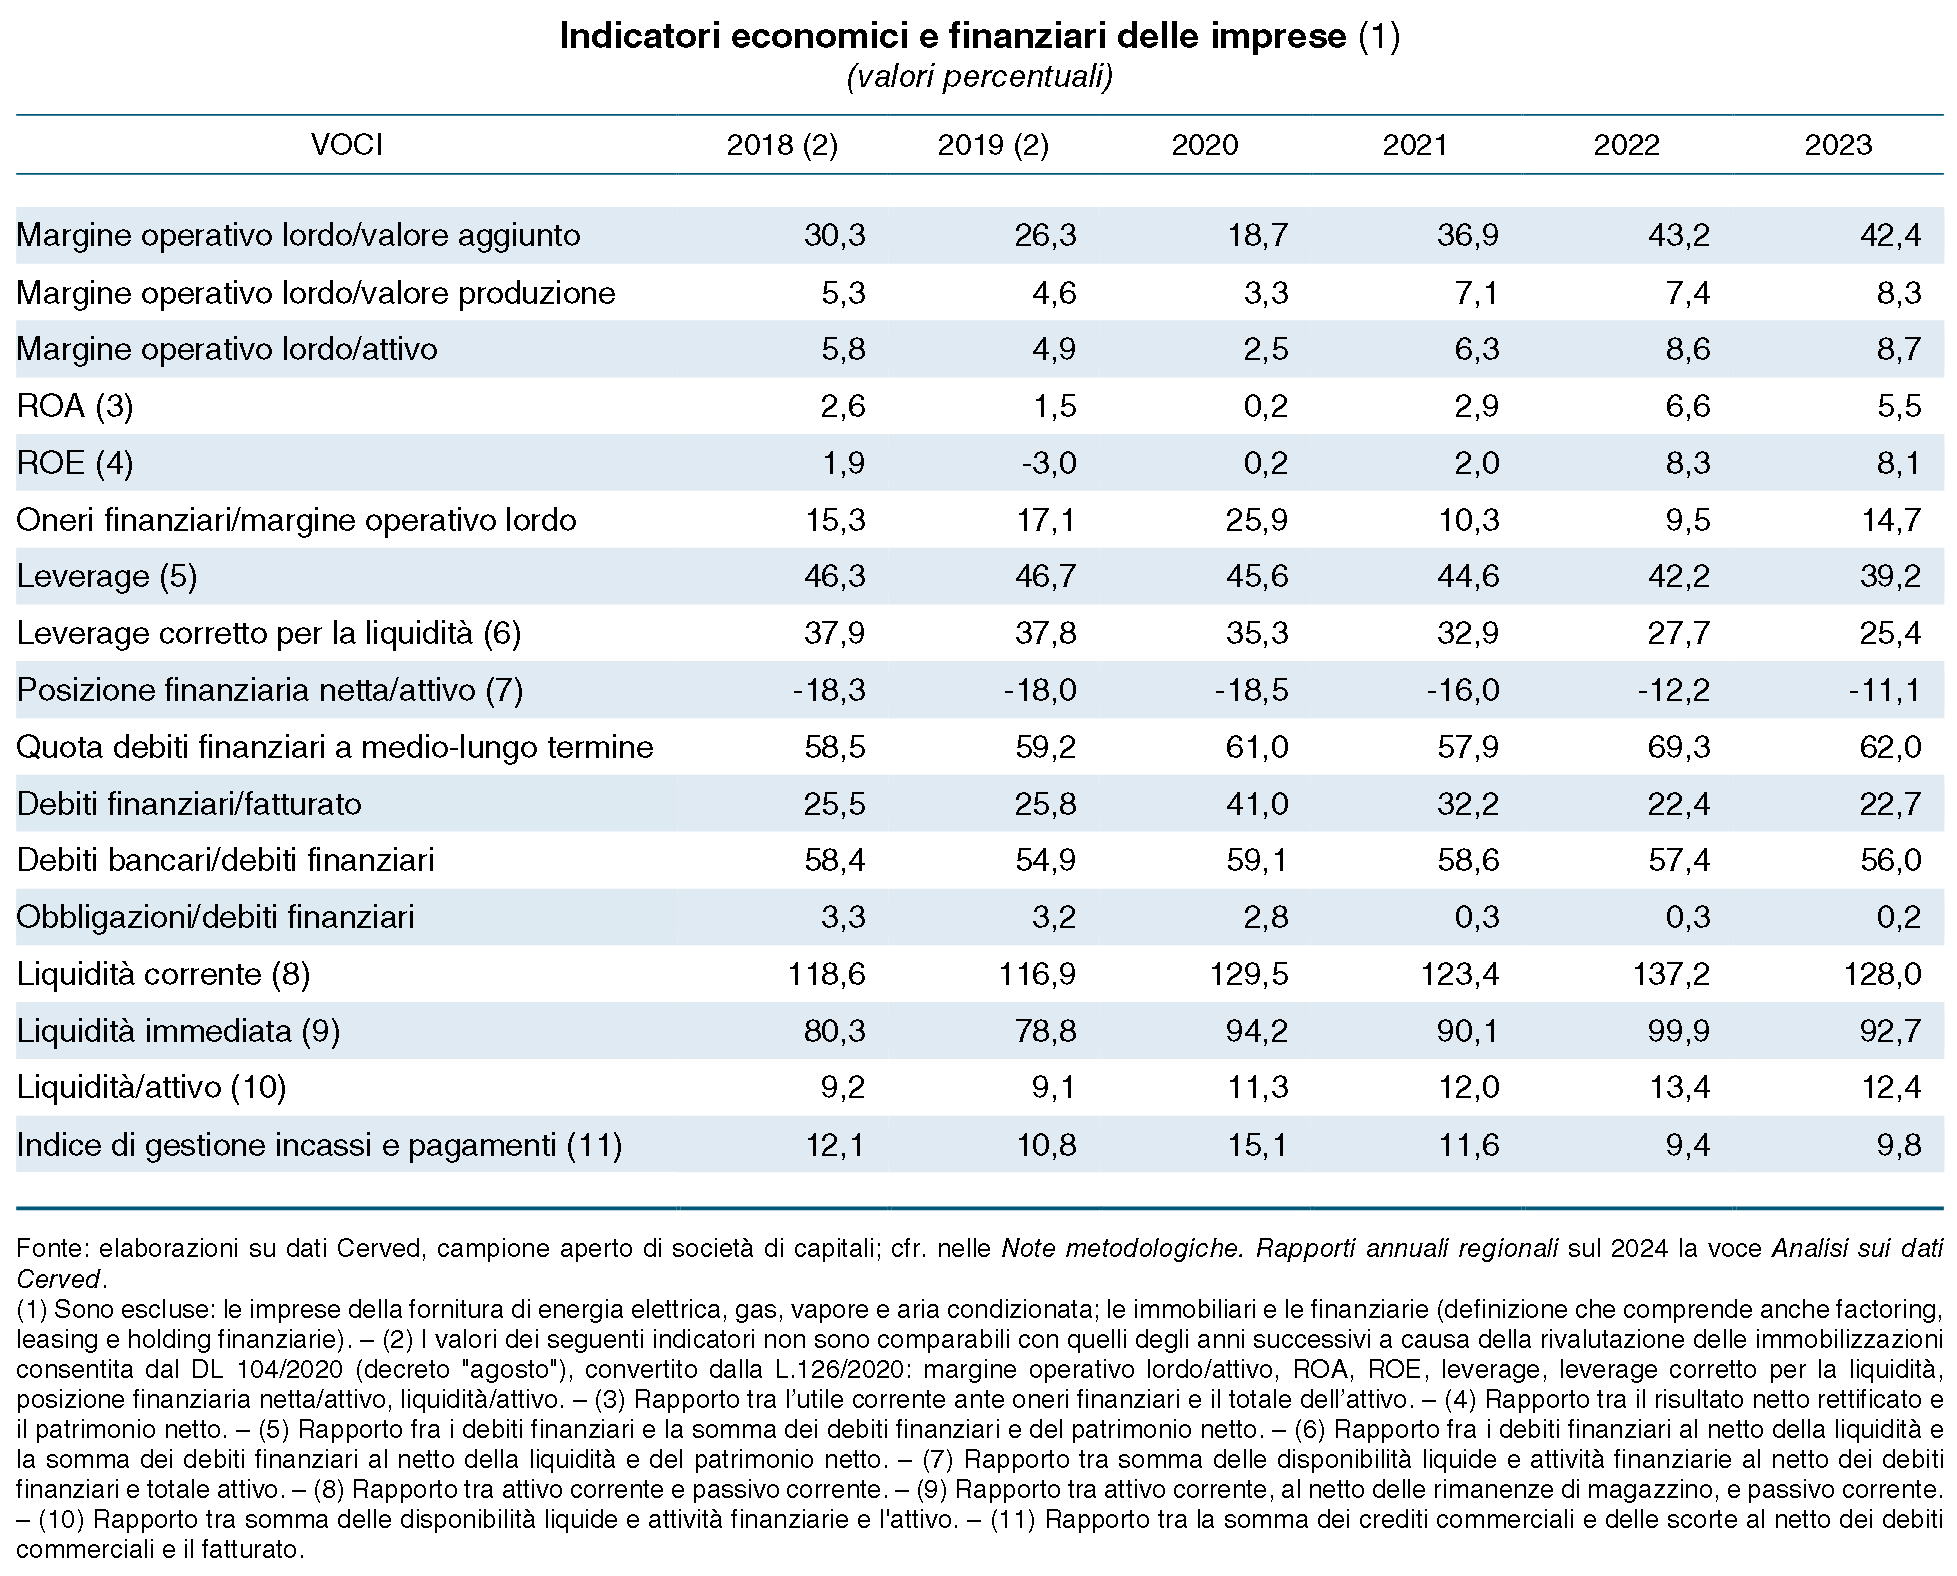
\includegraphics[keepaspectratio]{./media/immagine001.png}}

Il presente studio vuole analizzare l'andamento degli indicatori per
regione nel tempo.\\
Un focus viene fatto sul credit crunch.

\begin{center}\rule{0.5\linewidth}{0.5pt}\end{center}

\subsection{Dati}\label{dati}

\begin{Shaded}
\begin{Highlighting}[]
\ImportTok{import}\NormalTok{ pandas }\ImportTok{as}\NormalTok{ pd, os}
\NormalTok{os.chdir(}\StringTok{\textquotesingle{}D:/\textquotesingle{}}\NormalTok{)}
\NormalTok{file\_path }\OperatorTok{=} \StringTok{"Bankit\_ratios\_2025H1.tsv"}
\NormalTok{df }\OperatorTok{=}\NormalTok{ pd.read\_csv(file\_path, sep}\OperatorTok{=}\StringTok{"}\CharTok{\textbackslash{}t}\StringTok{"}\NormalTok{)}
\NormalTok{df.columns }\OperatorTok{=}\NormalTok{ [}\StringTok{"REGIONE"}\NormalTok{, }\StringTok{"RATIO"}\NormalTok{, }\StringTok{"ANNO"}\NormalTok{, }\StringTok{"VALORE"}\NormalTok{]}
\NormalTok{df[}\StringTok{"VALORE"}\NormalTok{] }\OperatorTok{=}\NormalTok{ df[}\StringTok{"VALORE"}\NormalTok{].}\BuiltInTok{str}\NormalTok{.replace(}\StringTok{","}\NormalTok{, }\StringTok{"."}\NormalTok{).astype(}\BuiltInTok{float}\NormalTok{)}
\NormalTok{mezzogiorno }\OperatorTok{=}\NormalTok{ \{}\StringTok{"ABR"}\NormalTok{, }\StringTok{"BAS"}\NormalTok{, }\StringTok{"CAL"}\NormalTok{, }\StringTok{"CAM"}\NormalTok{, }\StringTok{"PUG"}\NormalTok{, }\StringTok{"SAR"}\NormalTok{, }\StringTok{"SIC"}\NormalTok{, }\StringTok{"MOL"}\NormalTok{\}}
\NormalTok{df[}\StringTok{"MACROAREA"}\NormalTok{] }\OperatorTok{=}\NormalTok{ df[}\StringTok{"REGIONE"}\NormalTok{].}\BuiltInTok{apply}\NormalTok{(}\KeywordTok{lambda}\NormalTok{ x: }\StringTok{"Mezzogiorno"} \ControlFlowTok{if}\NormalTok{ x }\KeywordTok{in}\NormalTok{ mezzogiorno }\ControlFlowTok{else} \StringTok{"Centro{-}Nord"}\NormalTok{)}
\CommentTok{\# Calcolo della media per macroarea, ratio e anno}
\NormalTok{df\_grouped }\OperatorTok{=}\NormalTok{ df.groupby([}\StringTok{"MACROAREA"}\NormalTok{, }\StringTok{"RATIO"}\NormalTok{, }\StringTok{"ANNO"}\NormalTok{])[}\StringTok{"VALORE"}\NormalTok{].mean().reset\_index()}
\CommentTok{\# Pivot per confronto tra Mezzogiorno e Centro{-}Nord}
\NormalTok{df\_pivot }\OperatorTok{=}\NormalTok{ df\_grouped.pivot(index}\OperatorTok{=}\NormalTok{[}\StringTok{"RATIO"}\NormalTok{, }\StringTok{"ANNO"}\NormalTok{], columns}\OperatorTok{=}\StringTok{"MACROAREA"}\NormalTok{, values}\OperatorTok{=}\StringTok{"VALORE"}\NormalTok{).reset\_index()}
\NormalTok{df\_pivot}
\end{Highlighting}
\end{Shaded}

\subsubsection{Indicatori presenti}\label{indicatori-presenti}

Il dataset contiene rapporti finanziari chiave, tra cui:

\begin{itemize}
\tightlist
\item
  Debiti bancari / Debiti finanziari: incidenza dei prestiti bancari sul
  totale dei debiti finanziari.
\item
  Oneri finanziari / Valore della produzione: peso del costo del debito
  rispetto al fatturato.
\item
  Patrimonio netto / Totale delle passività: misura della solidità
  patrimoniale.
\item
  Indebitamento finanziario / Attivo: leva finanziaria.
\item
  Autofinanziamento / Investimenti: capacità interna di finanziare la
  crescita.
\end{itemize}

Le imprese del Mezzogiorno risultano più dipendenti dal credito
bancario, con struttura finanziaria più fragile e costo del debito più
elevato.

Ciò segnala un ritardo nell'accesso alla finanza alternativa e nella
capacità di autofinanziamento.

\subsubsection{Debiti bancari / Debiti
finanziari}\label{debiti-bancari-debiti-finanziari}

Costantemente più alto nel Mezzogiorno: segno che le imprese meridionali
fanno maggiormente ricorso al credito bancario tradizionale, con meno
accesso a strumenti alternativi (leasing, factoring, minibond).

Il gap è stabile: \textasciitilde10--15 punti percentuali a favore del
Centro-Nord.

\subsubsection{Oneri finanziari / Valore della
produzione}\label{oneri-finanziari-valore-della-produzione}

Più elevati nel Mezzogiorno, con un divario che si allarga nel
2022--2023.

Indica che il costo del denaro pesa di più per le imprese meridionali, a
parità di fatturato: possibile effetto combinato di rating più deboli,
minore concorrenza bancaria, meno strumenti di copertura.

\subsubsection{Patrimonio netto / Totale delle
passività}\label{patrimonio-netto-totale-delle-passivituxe0}

Centro-Nord meglio capitalizzato: rapporto stabilmente superiore, anche
in anni critici.

Le imprese del Sud mostrano una minore patrimonializzazione, quindi
maggiore vulnerabilità in caso di shock o aumento dei tassi.

\subsubsection{Autofinanziamento /
Investimenti}\label{autofinanziamento-investimenti}

Il Centro-Nord finanzia una quota più ampia degli investimenti con
risorse proprie.

Il Mezzogiorno mostra maggiore dipendenza da fonti esterne (pubbliche o
bancarie), che rende l'investimento più volatile.

\subsubsection{Evoluzione temporale
(2018--2023)}\label{evoluzione-temporale-20182023}

\begin{itemize}
\tightlist
\item
  Post-Covid (2020--2021): leggero miglioramento in molti indicatori,
  probabilmente per effetto di moratorie, liquidità straordinaria, fondo
  di garanzia.
\item
  2022--2023: inizia a emergere un deterioramento, con peggioramento
  degli oneri finanziari e lieve riduzione della patrimonializzazione.
\end{itemize}

\subsection{Cluster analysis}\label{cluster-analysis}

\phantomsection\label{fig1}
\begin{Shaded}
\begin{Highlighting}[]
\ImportTok{from}\NormalTok{ sklearn.preprocessing }\ImportTok{import}\NormalTok{ StandardScaler}
\ImportTok{from}\NormalTok{ sklearn.cluster }\ImportTok{import}\NormalTok{ KMeans}
\ImportTok{import}\NormalTok{ matplotlib.pyplot }\ImportTok{as}\NormalTok{ plt}
\CommentTok{\# === Preparazione dati: media 2018–2023 per regione e ratio}
\NormalTok{df\_cluster }\OperatorTok{=}\NormalTok{ df.groupby([}\StringTok{"REGIONE"}\NormalTok{, }\StringTok{"RATIO"}\NormalTok{])[}\StringTok{"VALORE"}\NormalTok{].mean().unstack()}

\CommentTok{\# === Rimozione regioni con valori NaN}
\NormalTok{df\_cluster\_clean }\OperatorTok{=}\NormalTok{ df\_cluster.dropna()}

\CommentTok{\# === Standardizzazione}
\NormalTok{scaler }\OperatorTok{=}\NormalTok{ StandardScaler()}
\NormalTok{X\_scaled\_clean }\OperatorTok{=}\NormalTok{ scaler.fit\_transform(df\_cluster\_clean)}

\CommentTok{\# === Metodo del gomito per scelta K ottimale}
\NormalTok{K\_range }\OperatorTok{=} \BuiltInTok{range}\NormalTok{(}\DecValTok{1}\NormalTok{, }\DecValTok{10}\NormalTok{)}
\NormalTok{inertia\_clean }\OperatorTok{=}\NormalTok{ []}
\ControlFlowTok{for}\NormalTok{ k }\KeywordTok{in}\NormalTok{ K\_range:}
\NormalTok{    kmeans }\OperatorTok{=}\NormalTok{ KMeans(n\_clusters}\OperatorTok{=}\NormalTok{k, random\_state}\OperatorTok{=}\DecValTok{0}\NormalTok{, n\_init}\OperatorTok{=}\DecValTok{10}\NormalTok{)}
\NormalTok{    kmeans.fit(X\_scaled\_clean)}
\NormalTok{    inertia\_clean.append(kmeans.inertia\_)}

\CommentTok{\# === Visualizzazione gomito}
\NormalTok{plt.figure(figsize}\OperatorTok{=}\NormalTok{(}\DecValTok{8}\NormalTok{, }\DecValTok{5}\NormalTok{))}
\NormalTok{plt.plot(K\_range, inertia\_clean, marker}\OperatorTok{=}\StringTok{\textquotesingle{}o\textquotesingle{}}\NormalTok{, color}\OperatorTok{=}\StringTok{\textquotesingle{}green\textquotesingle{}}\NormalTok{)}
\NormalTok{plt.xlabel(}\StringTok{"Numero di cluster (k)"}\NormalTok{)}
\NormalTok{plt.ylabel(}\StringTok{"Inertia"}\NormalTok{)}
\NormalTok{plt.title(}\StringTok{"Elbow curve"}\NormalTok{)}
\NormalTok{plt.grid(}\VariableTok{True}\NormalTok{)}
\NormalTok{plt.ylim(}\BuiltInTok{min}\NormalTok{(inertia\_clean) }\OperatorTok{*} \FloatTok{0.95}\NormalTok{, }\BuiltInTok{max}\NormalTok{(inertia\_clean) }\OperatorTok{*} \FloatTok{1.05}\NormalTok{)  }\CommentTok{\# zoom verticale}
\NormalTok{plt.show()}
\end{Highlighting}
\end{Shaded}

\begin{Shaded}
\begin{Highlighting}[]
\CommentTok{\# === Clustering finale (K=3)}
\NormalTok{kmeans\_final }\OperatorTok{=}\NormalTok{ KMeans(n\_clusters}\OperatorTok{=}\DecValTok{3}\NormalTok{, random\_state}\OperatorTok{=}\DecValTok{0}\NormalTok{, n\_init}\OperatorTok{=}\DecValTok{10}\NormalTok{)}

\CommentTok{\# Copia sicura per evitare ambiguità}
\NormalTok{df\_cluster\_clean }\OperatorTok{=}\NormalTok{ df\_cluster\_clean.copy()}
\NormalTok{df\_cluster\_clean[}\StringTok{"CLUSTER"}\NormalTok{] }\OperatorTok{=}\NormalTok{ kmeans\_final.fit\_predict(X\_scaled\_clean)}

\CommentTok{\# === Valori medi per cluster}
\CommentTok{\# Valori medi per cluster (trasposti)}
\NormalTok{df\_cluster\_mean }\OperatorTok{=}\NormalTok{ df\_cluster\_clean.groupby(}\StringTok{"CLUSTER"}\NormalTok{).mean().}\BuiltInTok{round}\NormalTok{(}\DecValTok{2}\NormalTok{)}
\NormalTok{df\_cluster\_mean\_t }\OperatorTok{=}\NormalTok{ df\_cluster\_mean.T.sort\_index()}

\CommentTok{\# Uso della libreria tabulate per mostrare una tabella ben formattata in stile "pretty"}
\ImportTok{from}\NormalTok{ tabulate }\ImportTok{import}\NormalTok{ tabulate}

\BuiltInTok{print}\NormalTok{(tabulate(df\_cluster\_mean\_t.reset\_index(), headers}\OperatorTok{=}\StringTok{"keys"}\NormalTok{, tablefmt}\OperatorTok{=}\StringTok{"github"}\NormalTok{, showindex}\OperatorTok{=}\VariableTok{False}\NormalTok{))}

\NormalTok{df\_cluster\_mean\_t.to\_html(}\StringTok{"cluster\_table.html"}\NormalTok{, float\_format}\OperatorTok{=}\StringTok{"}\SpecialCharTok{\%.2f}\StringTok{"}\NormalTok{)}
\end{Highlighting}
\end{Shaded}

La segmentazione delle regioni italiane in 3 cluster basata sui loro
indicatori finanziari medi (2018--2023). Ogni cluster rappresenta un
profilo omogeneo di comportamento finanziario:

\begin{itemize}
\tightlist
\item
  Cluster 0: regioni con alta dipendenza da debito bancario, leva
  moderata, e autofinanziamento medio.
\item
  Cluster 1: (da identificare dopo confronto completo) -- potenzialmente
  regioni con maggiore solidità patrimoniale.
\item
  Cluster 2: (da verificare) -- potrebbe contenere regioni con
  performance più efficienti o più fragili, a seconda della direzione
  dei ratios.
\end{itemize}

\begin{Shaded}
\begin{Highlighting}[]
\CommentTok{\# Eseguo il clustering con k=3}
\NormalTok{kmeans\_final }\OperatorTok{=}\NormalTok{ KMeans(n\_clusters}\OperatorTok{=}\DecValTok{3}\NormalTok{, random\_state}\OperatorTok{=}\DecValTok{0}\NormalTok{, n\_init}\OperatorTok{=}\DecValTok{10}\NormalTok{)}
\NormalTok{df\_cluster\_clean[}\StringTok{"CLUSTER"}\NormalTok{] }\OperatorTok{=}\NormalTok{ kmeans\_final.fit\_predict(X\_scaled\_clean)}

\CommentTok{\# Riordino per cluster}
\NormalTok{df\_cluster\_clean\_sorted }\OperatorTok{=}\NormalTok{ df\_cluster\_clean.sort\_values(}\StringTok{"CLUSTER"}\NormalTok{)}

\CommentTok{\# Visualizzo i risultati}
\NormalTok{df\_cluster\_clean\_sorted.reset\_index()}
\end{Highlighting}
\end{Shaded}

\subsubsection{🟢 Cluster 0: ``Alta dipendenza dal credito bancario'' -
Caratteristiche:}\label{cluster-0-alta-dipendenza-dal-credito-bancario---caratteristiche}

-Rapporto Debiti bancari\,/\,Debiti finanziari molto elevato. -Costi
finanziari / valore della produzione alti, segno di un onere del debito
significativo. -Leva finanziaria (Debiti finanziari / Attivo)
moderata-alta. -Autofinanziamento / Investimenti nella media: buona
capacità di generare risorse ma non sufficiente a coprire pienamente gli
investimenti. -Buona generazione di cassa, capacità applicativa di leva
Dipendenza da banche, vulnerabilità all'aumento tassi - Profilo: imprese
con forte esposizione al credito bancario, costi finanziari superiori
alla media, leva e autofinanziamento nella media

\subsubsection{🟡 Cluster 1: ``Solidità patrimoniale e rifinanziamento
bilanciato'' -
Caratteristiche:}\label{cluster-1-solidituxe0-patrimoniale-e-rifinanziamento-bilanciato---caratteristiche}

\begin{itemize}
\tightlist
\item
  Rapporto Patrimonio netto / Totale passività alto, indica buona
  capitalizzazione.
\item
  Debiti bancari / Debiti totali più contenuti rispetto al Cluster 0,
  con maggiore presenza di strumenti finanziari diversificati.
\item
  Autofinanziamento / Investimenti elevato: le imprese tendono a
  finanziare internamente gli investimenti.
\item
  Costi finanziari contenuti, in linea o al di sotto della media
  nazionale.
\item
  Elevata patrimonializzazione, autonomia finanziaria Potrebbe limitare
  leva utile per crescite aggressive
\item
  Profilo: imprese con maggiore capitale proprio, accesso più bilanciato
  alla finanza, migliore posizione finanziaria netta
\end{itemize}

\subsubsection{🔴 Cluster 2: ``Fragilità accentuata o piccole imprese
esposte'' -
Caratteristiche:}\label{cluster-2-fragilituxe0-accentuata-o-piccole-imprese-esposte---caratteristiche}

\begin{itemize}
\tightlist
\item
  Leva finanziaria molto elevata, indicando forte indebitamento.
\item
  Autofinanziamento / Investimenti basso: dipendenza significativa da
  finanziamenti esterni.
\item
  Rapporto Patrimonio netto / Totale passività più basso, indice di
  fragilità patrimoniale.
\item
  I costi finanziari possono essere molto alti, per l'effetto combinato
  di leva elevata e rating debole.
\item
  Possibile presenza di realtà dinamiche in espansione Elevata
  vulnerabilità finanziaria, rischi elevati
\item
  Profilo: combinazione di leve elevate, bassa patrimonializzazione,
  autofinanziamento ridotto -- possibili anomalie strutturali o effetti
  della dimensione media d'impresa
\end{itemize}

\phantomsection\label{fig3}
\begin{Shaded}
\begin{Highlighting}[]
\CommentTok{\# Generazione di un radar unico con tutti i cluster sovrapposti}

\ImportTok{import}\NormalTok{ numpy }\ImportTok{as}\NormalTok{ np}
\NormalTok{labels }\OperatorTok{=}\NormalTok{ df\_cluster\_mean\_t.index.tolist()}
\NormalTok{num\_vars }\OperatorTok{=} \BuiltInTok{len}\NormalTok{(labels)}
\NormalTok{angles }\OperatorTok{=}\NormalTok{ np.linspace(}\DecValTok{0}\NormalTok{, }\DecValTok{2} \OperatorTok{*}\NormalTok{ np.pi, num\_vars, endpoint}\OperatorTok{=}\VariableTok{False}\NormalTok{).tolist()}
\NormalTok{angles }\OperatorTok{+=}\NormalTok{ angles[:}\DecValTok{1}\NormalTok{]}

\CommentTok{\# Cluster colors e labels}
\NormalTok{cluster\_colors }\OperatorTok{=}\NormalTok{ [}\StringTok{\textquotesingle{}gold\textquotesingle{}}\NormalTok{, }\StringTok{\textquotesingle{}green\textquotesingle{}}\NormalTok{, }\StringTok{\textquotesingle{}red\textquotesingle{}}\NormalTok{]}
\NormalTok{cluster\_labels }\OperatorTok{=}\NormalTok{ [}\StringTok{\textquotesingle{}Cluster 0\textquotesingle{}}\NormalTok{, }\StringTok{\textquotesingle{}Cluster 1\textquotesingle{}}\NormalTok{, }\StringTok{\textquotesingle{}Cluster 2\textquotesingle{}}\NormalTok{]}

\CommentTok{\# Radar comparativo senza riempimento interno e con immagine più grande}

\NormalTok{fig, ax }\OperatorTok{=}\NormalTok{ plt.subplots(figsize}\OperatorTok{=}\NormalTok{(}\DecValTok{12}\NormalTok{,}\DecValTok{12}\NormalTok{), subplot\_kw}\OperatorTok{=}\BuiltInTok{dict}\NormalTok{(polar}\OperatorTok{=}\VariableTok{True}\NormalTok{))}

\ControlFlowTok{for}\NormalTok{ i }\KeywordTok{in} \BuiltInTok{range}\NormalTok{(}\DecValTok{3}\NormalTok{):}
\NormalTok{    values }\OperatorTok{=}\NormalTok{ df\_cluster\_mean\_t.iloc[:, i].tolist()}
\NormalTok{    values }\OperatorTok{+=}\NormalTok{ values[:}\DecValTok{1}\NormalTok{]}
\NormalTok{    ax.plot(angles, values, color}\OperatorTok{=}\NormalTok{cluster\_colors[i], linewidth}\OperatorTok{=}\DecValTok{2}\NormalTok{, label}\OperatorTok{=}\NormalTok{cluster\_labels[i])}
    \CommentTok{\# Niente fill per maggiore pulizia visiva}

\NormalTok{ax.set\_xticks(angles[:}\OperatorTok{{-}}\DecValTok{1}\NormalTok{])}
\NormalTok{ax.set\_xticklabels(labels, fontsize}\OperatorTok{=}\DecValTok{10}\NormalTok{)}
\NormalTok{ax.set\_yticklabels([])}
\NormalTok{ax.set\_title(}\StringTok{"Grafico Radar dei Cluster"}\NormalTok{, fontsize}\OperatorTok{=}\DecValTok{16}\NormalTok{, pad}\OperatorTok{=}\DecValTok{20}\NormalTok{)}
\NormalTok{ax.legend(loc}\OperatorTok{=}\StringTok{\textquotesingle{}upper right\textquotesingle{}}\NormalTok{, bbox\_to\_anchor}\OperatorTok{=}\NormalTok{(}\FloatTok{1.3}\NormalTok{, }\FloatTok{1.1}\NormalTok{))}

\NormalTok{plt.tight\_layout()}
\NormalTok{plt.show()}
\end{Highlighting}
\end{Shaded}

\begin{Shaded}
\begin{Highlighting}[]
\CommentTok{\# Estraggo le regioni per ciascun cluster}
\NormalTok{cluster\_regioni }\OperatorTok{=}\NormalTok{ df\_cluster\_clean\_sorted.reset\_index()[[}\StringTok{"REGIONE"}\NormalTok{, }\StringTok{"CLUSTER"}\NormalTok{]]}
\NormalTok{cluster\_regioni\_grouped }\OperatorTok{=}\NormalTok{ cluster\_regioni.groupby(}\StringTok{"CLUSTER"}\NormalTok{)[}\StringTok{"REGIONE"}\NormalTok{].}\BuiltInTok{apply}\NormalTok{(}\BuiltInTok{list}\NormalTok{).reset\_index(name}\OperatorTok{=}\StringTok{"REGIONI"}\NormalTok{)}

\NormalTok{cluster\_regioni\_grouped}
\end{Highlighting}
\end{Shaded}

\phantomsection\label{fig2}
\begin{Shaded}
\begin{Highlighting}[]
\ImportTok{import}\NormalTok{ geopandas }\ImportTok{as}\NormalTok{ gpd}
\ImportTok{import}\NormalTok{ matplotlib.pyplot }\ImportTok{as}\NormalTok{ plt}

\CommentTok{\# Uso un dataset di regioni italiane semplificato da ISTAT (necessario importarlo)}
\CommentTok{\# Carico un dataset esterno con codici e geometrie regionali}
\NormalTok{regioni }\OperatorTok{=}\NormalTok{ gpd.read\_file(}\StringTok{"https://raw.githubusercontent.com/openpolis/geojson{-}italy/master/geojson/limits\_IT\_regions.geojson"}\NormalTok{)}

\CommentTok{\# Mappo i codici ISO (es. \textquotesingle{}IT{-}62\textquotesingle{}) in codici del file (es. \textquotesingle{}VEN\textquotesingle{}) usando una tabella}
\NormalTok{codici\_regioni }\OperatorTok{=}\NormalTok{ \{}
    \StringTok{\textquotesingle{}Abruzzo\textquotesingle{}}\NormalTok{: }\StringTok{\textquotesingle{}ABR\textquotesingle{}}\NormalTok{, }\StringTok{\textquotesingle{}Basilicata\textquotesingle{}}\NormalTok{: }\StringTok{\textquotesingle{}BAS\textquotesingle{}}\NormalTok{, }\StringTok{\textquotesingle{}Calabria\textquotesingle{}}\NormalTok{: }\StringTok{\textquotesingle{}CAL\textquotesingle{}}\NormalTok{, }\StringTok{\textquotesingle{}Campania\textquotesingle{}}\NormalTok{: }\StringTok{\textquotesingle{}CAM\textquotesingle{}}\NormalTok{,}
    \StringTok{\textquotesingle{}Emilia{-}Romagna\textquotesingle{}}\NormalTok{: }\StringTok{\textquotesingle{}EMR\textquotesingle{}}\NormalTok{, }\StringTok{\textquotesingle{}Friuli{-}Venezia Giulia\textquotesingle{}}\NormalTok{: }\StringTok{\textquotesingle{}FVG\textquotesingle{}}\NormalTok{, }\StringTok{\textquotesingle{}Lazio\textquotesingle{}}\NormalTok{: }\StringTok{\textquotesingle{}LAZ\textquotesingle{}}\NormalTok{, }\StringTok{\textquotesingle{}Liguria\textquotesingle{}}\NormalTok{: }\StringTok{\textquotesingle{}LIG\textquotesingle{}}\NormalTok{,}
    \StringTok{\textquotesingle{}Lombardia\textquotesingle{}}\NormalTok{: }\StringTok{\textquotesingle{}LOM\textquotesingle{}}\NormalTok{, }\StringTok{\textquotesingle{}Marche\textquotesingle{}}\NormalTok{: }\StringTok{\textquotesingle{}MAR\textquotesingle{}}\NormalTok{, }\StringTok{\textquotesingle{}Molise\textquotesingle{}}\NormalTok{: }\StringTok{\textquotesingle{}MOL\textquotesingle{}}\NormalTok{, }\StringTok{\textquotesingle{}Piemonte\textquotesingle{}}\NormalTok{: }\StringTok{\textquotesingle{}PIE\textquotesingle{}}\NormalTok{, }\StringTok{\textquotesingle{}Puglia\textquotesingle{}}\NormalTok{: }\StringTok{\textquotesingle{}PUG\textquotesingle{}}\NormalTok{,}
    \StringTok{\textquotesingle{}Sardegna\textquotesingle{}}\NormalTok{: }\StringTok{\textquotesingle{}SAR\textquotesingle{}}\NormalTok{, }\StringTok{\textquotesingle{}Sicilia\textquotesingle{}}\NormalTok{: }\StringTok{\textquotesingle{}SIC\textquotesingle{}}\NormalTok{, }\StringTok{\textquotesingle{}Toscana\textquotesingle{}}\NormalTok{: }\StringTok{\textquotesingle{}TOS\textquotesingle{}}\NormalTok{, }\StringTok{\textquotesingle{}Trentino{-}Alto Adige/Südtirol\textquotesingle{}}\NormalTok{: }\StringTok{\textquotesingle{}Tre\textquotesingle{}}\NormalTok{,}
    \StringTok{\textquotesingle{}Umbria\textquotesingle{}}\NormalTok{: }\StringTok{\textquotesingle{}UMB\textquotesingle{}}\NormalTok{, }\StringTok{\textquotesingle{}Valle d}\CharTok{\textbackslash{}\textquotesingle{}}\StringTok{Aosta/Vallée d}\CharTok{\textbackslash{}\textquotesingle{}}\StringTok{Aoste\textquotesingle{}}\NormalTok{: }\StringTok{\textquotesingle{}VAO\textquotesingle{}}\NormalTok{, }\StringTok{\textquotesingle{}Veneto\textquotesingle{}}\NormalTok{: }\StringTok{\textquotesingle{}VEN\textquotesingle{}}\NormalTok{,}
    \StringTok{\textquotesingle{}Provincia Autonoma Bolzano/Bozen\textquotesingle{}}\NormalTok{: }\StringTok{\textquotesingle{}Bol\textquotesingle{}}
\NormalTok{\}}

\NormalTok{regioni[}\StringTok{"CODICE"}\NormalTok{] }\OperatorTok{=}\NormalTok{ regioni[}\StringTok{"reg\_name"}\NormalTok{].}\BuiltInTok{map}\NormalTok{(codici\_regioni)}

\CommentTok{\# Unisco i cluster alle geometrie}
\NormalTok{df\_map }\OperatorTok{=}\NormalTok{ df\_cluster\_clean\_sorted.reset\_index()[[}\StringTok{"REGIONE"}\NormalTok{, }\StringTok{"CLUSTER"}\NormalTok{]]}
\NormalTok{mappa\_cluster }\OperatorTok{=}\NormalTok{ regioni.merge(df\_map, left\_on}\OperatorTok{=}\StringTok{"CODICE"}\NormalTok{, right\_on}\OperatorTok{=}\StringTok{"REGIONE"}\NormalTok{, how}\OperatorTok{=}\StringTok{"left"}\NormalTok{)}

\ImportTok{from}\NormalTok{ matplotlib.colors }\ImportTok{import}\NormalTok{ ListedColormap}
\CommentTok{\# Plot}
\NormalTok{fig, ax }\OperatorTok{=}\NormalTok{ plt.subplots(}\DecValTok{1}\NormalTok{, }\DecValTok{1}\NormalTok{, figsize}\OperatorTok{=}\NormalTok{(}\DecValTok{10}\NormalTok{, }\DecValTok{12}\NormalTok{))}
\NormalTok{cmap3 }\OperatorTok{=}\NormalTok{ ListedColormap([}\StringTok{"\#FFD700"}\NormalTok{, }\StringTok{"\#228B22"}\NormalTok{, }\StringTok{"\#B22222"}\NormalTok{])  }\CommentTok{\# giallo, verde, rosso}
\NormalTok{mappa\_cluster.plot(}
\NormalTok{    column}\OperatorTok{=}\StringTok{"CLUSTER"}\NormalTok{,}
\NormalTok{    cmap}\OperatorTok{=}\NormalTok{cmap3,}
\NormalTok{    linewidth}\OperatorTok{=}\FloatTok{0.8}\NormalTok{,}
\NormalTok{    edgecolor}\OperatorTok{=}\StringTok{"gray"}\NormalTok{,}
\NormalTok{    legend}\OperatorTok{=}\VariableTok{False}\NormalTok{,}
\NormalTok{    ax}\OperatorTok{=}\NormalTok{ax}
\NormalTok{)}
\NormalTok{ax.set\_title(}\StringTok{"Cluster finanziari delle regioni italiane (2018–2023)"}\NormalTok{, fontsize}\OperatorTok{=}\DecValTok{14}\NormalTok{)}
\NormalTok{ax.axis(}\StringTok{"off"}\NormalTok{)}
\NormalTok{plt.show()}
\end{Highlighting}
\end{Shaded}

\subsection{Analisi temporale}\label{analisi-temporale}

Rifacciamo il clustering considerando tutte le annualità (2018--2023)
per ogni ratio, quindi: - Ogni regione è descritta da 103 variabili
(ratio\_anno), invece della sola media. - Il clustering cattura anche la
dinamica temporale e non solo il valore medio statico. - Le regioni sono
classificate in 3 cluster più coerenti con l'evoluzione nel tempo degli
indicatori.

\begin{Shaded}
\begin{Highlighting}[]
\ImportTok{import}\NormalTok{ pandas }\ImportTok{as}\NormalTok{ pd}
\NormalTok{file\_path }\OperatorTok{=} \StringTok{"D:/Bankit\_ratios\_2025H1.tsv"}
\NormalTok{df }\OperatorTok{=}\NormalTok{ pd.read\_csv(file\_path, sep}\OperatorTok{=}\StringTok{"}\CharTok{\textbackslash{}t}\StringTok{"}\NormalTok{)}
\NormalTok{df.columns }\OperatorTok{=}\NormalTok{ [}\StringTok{"REGIONE"}\NormalTok{, }\StringTok{"RATIO"}\NormalTok{, }\StringTok{"ANNO"}\NormalTok{, }\StringTok{"VALORE"}\NormalTok{]}
\NormalTok{df[}\StringTok{"VALORE"}\NormalTok{] }\OperatorTok{=}\NormalTok{ df[}\StringTok{"VALORE"}\NormalTok{].}\BuiltInTok{str}\NormalTok{.replace(}\StringTok{","}\NormalTok{, }\StringTok{"."}\NormalTok{).astype(}\BuiltInTok{float}\NormalTok{)}
\CommentTok{\# Pivot table: una colonna per ciascun ratio\_anno}
\NormalTok{df[}\StringTok{"RATIO\_ANNO"}\NormalTok{] }\OperatorTok{=}\NormalTok{ df[}\StringTok{"RATIO"}\NormalTok{] }\OperatorTok{+} \StringTok{"\_"} \OperatorTok{+}\NormalTok{ df[}\StringTok{"ANNO"}\NormalTok{].astype(}\BuiltInTok{str}\NormalTok{)}
\NormalTok{df\_wide }\OperatorTok{=}\NormalTok{ df.pivot(index}\OperatorTok{=}\StringTok{"REGIONE"}\NormalTok{, columns}\OperatorTok{=}\StringTok{"RATIO\_ANNO"}\NormalTok{, values}\OperatorTok{=}\StringTok{"VALORE"}\NormalTok{)}

\CommentTok{\# Rimuovo righe con NaN e standardizzo}
\NormalTok{df\_wide\_clean }\OperatorTok{=}\NormalTok{ df\_wide.dropna().copy()}
\NormalTok{scaler }\OperatorTok{=}\NormalTok{ StandardScaler()}
\NormalTok{X\_scaled\_all\_years }\OperatorTok{=}\NormalTok{ scaler.fit\_transform(df\_wide\_clean)}

\CommentTok{\# Clustering}
\NormalTok{kmeans\_all\_years }\OperatorTok{=}\NormalTok{ KMeans(n\_clusters}\OperatorTok{=}\DecValTok{3}\NormalTok{, random\_state}\OperatorTok{=}\DecValTok{0}\NormalTok{, n\_init}\OperatorTok{=}\DecValTok{10}\NormalTok{)}
\NormalTok{df\_wide\_clean[}\StringTok{"CLUSTER"}\NormalTok{] }\OperatorTok{=}\NormalTok{ kmeans\_all\_years.fit\_predict(X\_scaled\_all\_years)}

\CommentTok{\# Salvo la tabella finale}
\NormalTok{df\_cluster\_all\_years }\OperatorTok{=}\NormalTok{ df\_wide\_clean.copy()}

\CommentTok{\# Recupero il DataFrame originale}
\NormalTok{df\_clusters\_by\_year }\OperatorTok{=}\NormalTok{ df.copy()}

\CommentTok{\# Aggiungo la colonna cluster da df\_cluster\_all\_years}
\NormalTok{cluster\_map }\OperatorTok{=}\NormalTok{ df\_cluster\_all\_years[}\StringTok{"CLUSTER"}\NormalTok{]}
\NormalTok{df\_clusters\_by\_year[}\StringTok{"CLUSTER"}\NormalTok{] }\OperatorTok{=}\NormalTok{ df\_clusters\_by\_year[}\StringTok{"REGIONE"}\NormalTok{].}\BuiltInTok{map}\NormalTok{(cluster\_map)}

\CommentTok{\# Tabella finale: regioni in riga, anni in colonna, valore = cluster}
\NormalTok{df\_cluster\_matrix }\OperatorTok{=}\NormalTok{ df\_clusters\_by\_year[[}\StringTok{"REGIONE"}\NormalTok{, }\StringTok{"ANNO"}\NormalTok{, }\StringTok{"CLUSTER"}\NormalTok{]].drop\_duplicates()}
\NormalTok{df\_cluster\_matrix\_wide }\OperatorTok{=}\NormalTok{ df\_cluster\_matrix.pivot(index}\OperatorTok{=}\StringTok{"REGIONE"}\NormalTok{, columns}\OperatorTok{=}\StringTok{"ANNO"}\NormalTok{, values}\OperatorTok{=}\StringTok{"CLUSTER"}\NormalTok{).astype(}\StringTok{"Int64"}\NormalTok{)}

\NormalTok{df\_cluster\_matrix\_wide}
\end{Highlighting}
\end{Shaded}

\begin{Shaded}
\begin{Highlighting}[]
\ImportTok{import}\NormalTok{ pandas }\ImportTok{as}\NormalTok{ pd}
\ImportTok{import}\NormalTok{ numpy }\ImportTok{as}\NormalTok{ np}
\ImportTok{import}\NormalTok{ matplotlib.pyplot }\ImportTok{as}\NormalTok{ plt}
\ImportTok{from}\NormalTok{ sklearn.preprocessing }\ImportTok{import}\NormalTok{ StandardScaler}
\ImportTok{from}\NormalTok{ sklearn.cluster }\ImportTok{import}\NormalTok{ KMeans}

\CommentTok{\# === Caricamento e pulizia dati ===}
\NormalTok{df }\OperatorTok{=}\NormalTok{ pd.read\_csv(}\StringTok{"D:/Bankit\_ratios\_2025H1.tsv"}\NormalTok{, sep}\OperatorTok{=}\StringTok{"}\CharTok{\textbackslash{}t}\StringTok{"}\NormalTok{)}
\NormalTok{df.columns }\OperatorTok{=}\NormalTok{ [}\StringTok{"REGIONE"}\NormalTok{, }\StringTok{"RATIO"}\NormalTok{, }\StringTok{"ANNO"}\NormalTok{, }\StringTok{"VALORE"}\NormalTok{]}
\NormalTok{df[}\StringTok{"ANNO"}\NormalTok{] }\OperatorTok{=}\NormalTok{ df[}\StringTok{"ANNO"}\NormalTok{].}\BuiltInTok{str}\NormalTok{.replace(}\StringTok{"Y"}\NormalTok{, }\StringTok{""}\NormalTok{)}
\NormalTok{df[}\StringTok{"VALORE"}\NormalTok{] }\OperatorTok{=}\NormalTok{ df[}\StringTok{"VALORE"}\NormalTok{].}\BuiltInTok{str}\NormalTok{.replace(}\StringTok{","}\NormalTok{, }\StringTok{"."}\NormalTok{).astype(}\BuiltInTok{float}\NormalTok{)}
\CommentTok{\# === Filtro dati 2018 ===}
\NormalTok{df\_2018 }\OperatorTok{=}\NormalTok{ df[df[}\StringTok{"ANNO"}\NormalTok{] }\OperatorTok{==} \StringTok{"2018"}\NormalTok{]}

\CommentTok{\# === Pivot Regione x RATIO ===}
\NormalTok{df\_2018\_pivot }\OperatorTok{=}\NormalTok{ df\_2018.pivot(index}\OperatorTok{=}\StringTok{"REGIONE"}\NormalTok{, columns}\OperatorTok{=}\StringTok{"RATIO"}\NormalTok{, values}\OperatorTok{=}\StringTok{"VALORE"}\NormalTok{)}

\CommentTok{\# === Imputazione media colonna per valori mancanti ===}
\NormalTok{df\_2018\_pivot\_filled }\OperatorTok{=}\NormalTok{ df\_2018\_pivot.fillna(df\_2018\_pivot.mean(numeric\_only}\OperatorTok{=}\VariableTok{True}\NormalTok{))}

\CommentTok{\# === Standardizzazione e clustering (K=3) ===}
\NormalTok{scaler }\OperatorTok{=}\NormalTok{ StandardScaler()}
\NormalTok{X\_scaled }\OperatorTok{=}\NormalTok{ scaler.fit\_transform(df\_2018\_pivot\_filled)}

\NormalTok{kmeans }\OperatorTok{=}\NormalTok{ KMeans(n\_clusters}\OperatorTok{=}\DecValTok{3}\NormalTok{, random\_state}\OperatorTok{=}\DecValTok{0}\NormalTok{, n\_init}\OperatorTok{=}\DecValTok{10}\NormalTok{)}
\NormalTok{df\_2018\_pivot\_filled[}\StringTok{"CLUSTER"}\NormalTok{] }\OperatorTok{=}\NormalTok{ kmeans.fit\_predict(X\_scaled)}

\CommentTok{\# === Calcolo delle medie per cluster ===}
\NormalTok{df\_cluster\_mean\_2018 }\OperatorTok{=}\NormalTok{ df\_2018\_pivot\_filled.groupby(}\StringTok{"CLUSTER"}\NormalTok{).mean().T}

\CommentTok{\# === Definizione grafico radar ===}
\NormalTok{cluster\_colors }\OperatorTok{=}\NormalTok{ [}\StringTok{\textquotesingle{}gold\textquotesingle{}}\NormalTok{, }\StringTok{\textquotesingle{}green\textquotesingle{}}\NormalTok{, }\StringTok{\textquotesingle{}red\textquotesingle{}}\NormalTok{]}
\NormalTok{cluster\_labels }\OperatorTok{=}\NormalTok{ [}\StringTok{\textquotesingle{}Cluster 0\textquotesingle{}}\NormalTok{, }\StringTok{\textquotesingle{}Cluster 1\textquotesingle{}}\NormalTok{, }\StringTok{\textquotesingle{}Cluster 2\textquotesingle{}}\NormalTok{]}
\NormalTok{labels }\OperatorTok{=}\NormalTok{ df\_cluster\_mean\_2018.index.tolist()}
\NormalTok{num\_vars }\OperatorTok{=} \BuiltInTok{len}\NormalTok{(labels)}
\NormalTok{angles }\OperatorTok{=}\NormalTok{ np.linspace(}\DecValTok{0}\NormalTok{, }\DecValTok{2} \OperatorTok{*}\NormalTok{ np.pi, num\_vars, endpoint}\OperatorTok{=}\VariableTok{False}\NormalTok{).tolist()}
\NormalTok{angles }\OperatorTok{+=}\NormalTok{ angles[:}\DecValTok{1}\NormalTok{]}

\CommentTok{\# === Creazione radar chart ===}
\NormalTok{fig, ax }\OperatorTok{=}\NormalTok{ plt.subplots(figsize}\OperatorTok{=}\NormalTok{(}\DecValTok{14}\NormalTok{, }\DecValTok{14}\NormalTok{), subplot\_kw}\OperatorTok{=}\BuiltInTok{dict}\NormalTok{(polar}\OperatorTok{=}\VariableTok{True}\NormalTok{))}

\ControlFlowTok{for}\NormalTok{ i }\KeywordTok{in} \BuiltInTok{range}\NormalTok{(}\DecValTok{3}\NormalTok{):}
\NormalTok{    values }\OperatorTok{=}\NormalTok{ df\_cluster\_mean\_2018.iloc[:, i].tolist()}
\NormalTok{    values }\OperatorTok{+=}\NormalTok{ values[:}\DecValTok{1}\NormalTok{]}
\NormalTok{    ax.plot(angles, values, color}\OperatorTok{=}\NormalTok{cluster\_colors[i], linewidth}\OperatorTok{=}\DecValTok{2}\NormalTok{, label}\OperatorTok{=}\NormalTok{cluster\_labels[i])}

\NormalTok{ax.set\_xticks(angles[:}\OperatorTok{{-}}\DecValTok{1}\NormalTok{])}
\NormalTok{ax.set\_xticklabels(labels, fontsize}\OperatorTok{=}\DecValTok{9}\NormalTok{)}
\NormalTok{ax.set\_yticklabels([])}
\NormalTok{ax.set\_title(}\StringTok{"Grafico Radar dei Cluster {-} Anno 2018 (dati completati)"}\NormalTok{, fontsize}\OperatorTok{=}\DecValTok{16}\NormalTok{, pad}\OperatorTok{=}\DecValTok{20}\NormalTok{)}
\NormalTok{ax.legend(loc}\OperatorTok{=}\StringTok{\textquotesingle{}upper right\textquotesingle{}}\NormalTok{, bbox\_to\_anchor}\OperatorTok{=}\NormalTok{(}\FloatTok{1.3}\NormalTok{, }\FloatTok{1.1}\NormalTok{))}

\NormalTok{plt.tight\_layout()}
\NormalTok{plt.show()}
\end{Highlighting}
\end{Shaded}





\end{document}
